% !TEX root = ../thesis.tex
% compare covariance functions and generalization
% @author Tobias Wulf
%

\section{Vergleich der Kovarianzfunktionen und einsetzende Generalisierung}\label{sec:exp1}

\textbf{Zweck:} Als Vergleich der beiden implementierten Kernel-Module sollen ihre Kovarianzfunktionen und Eigenschaft zur Generalisierung bei einfacher Parametrierung untersucht werden. Ziel ist es, im besten Fall die Implementierung über die euklidische Abstandsfunktion nutzen zu können. Es würde sich dadurch eine Ressourcenersparnis in Bezug auf Speicherkapazität einstellen, da sich mit diesen Kernel Modelltrainingsdaten aus zwei eindimensionalen Vektoren bilden, statt dreidimensionaler Matrizen für die Kernel-Implementierung aus den Vorarbeiten. Diese nutzt als Abstandsfunktion die Frobenius Norm, siehe \autoref{eq:kfun}.


\clearpage


\textbf{Durchführung:} Es werden beide Kernel-Module nacheinander im Skript geladen und mit variierenden Parametern initialisiert. Die resultierenden Modelle werden ohne weitere Optimierungen betrieben, um grundlegende Eigenschaften der Kovarianzfunktionen und Generalisierung miteinander vergleichbar zu machen. Dabei wird eine Trainingsdatensatz verwendet der eine relative hohe Anzahl an Trainingspunkten $>50$ besitzt, dass der fehlenden Optimierung z.T. entgegenwirken soll. Die variierende Parametrierung der Kovarianzfunktionen in Längen- $\sigma_l$ und Höhenskalierung $\sigma_f^2$ wird für beide Kernel gleich durchgeführt. Im Anschluss werden Generalisierungseigenschaften mit den Modellen aus variierender Längenskalierung verglichen, um eine erste Abschätzung zur Modellkomplexität beobachten zu können.

\textbf{Erzeugte Datensätze:} Jeweils ein Trainings- und Testdatensatz mit korrespondierender Position des Sensors und Verkippungswinkel des Magneten.

\textbf{Matlab-Skript:} compareGPRKernels.m, siehe \autoref{mcode:comparegprkernels}.

\textbf{Abweichende Parameter von \autoref{tab:sim-params-exp}:}

\vspace{5mm}
\begin{table}[hp]
	\centering
	\resizebox{\textwidth}{!}{
		\begin{tabular}{l l c l}
			\toprule
			\textbf{Parametergruppe} & \textbf{Parameter} & \textbf{Wert}                                            & \textbf{Kurzbeschreibung}                 \\ \midrule
			TrainingOptions          & nAngles            & $56$                                                     & Anzahl gleichverteilter Simulationswinkel \\ \hline
			GPROptions               & kernel             & 'QFC'/ 'QFCAPX                                           & Kernel-Indikator variiert                 \\
			                         & $\theta$           & $\theta_1 = 1$, $\theta_2 = \left[ 1; 0,5; 2; 4 \right]$ & Kernel-Parametervektor, Variation 1       \\
			                         & $\theta$           & $\theta_1 = \left[ 1; 0,5; 2; 4 \right]$, $\theta_2 = 1$ & Kernel-Parametervektor, Variation 2       \\ \bottomrule
		\end{tabular}}
	\caption{Abweichende Simulationsparameter im Experiment zur Kovarianzfunktion.}
	\label{tab:params-exp1}
\end{table}


\clearpage


\textbf{Ergebnisse:} Die Ergebnisse des Experiments sind grafisch ausgewertet. \autoref{fig:vergleich-kovarianzfunktionen} zeigt das Verhalten der Kovarianzfunktionen bei variierender Skalierung über die Kernel-Parameter $\theta = (\sigma_f^2, \sigma_l)$, siehe \autoref{eq:kparam}. In \autoref{fig:vergleich-kovarianzmatrizen} sind resultierend Kovarianzmatrizen mit ausgeschalteter Skalierung für $\theta = (1, 1)$ gegenübergestellt. Die \autoref{fig:vergleich-qfc-sll} und \autoref{fig:vergleich-qfcapx-sll} zeigen die sich einstellenden Modellgeneralisierungen für beide Kernel-Varianten bei einfacher Längenskalierung der Kovarianzfunktionen über $\theta_2 = \sigma_l$. Die Höhenskalierung ist an dieser Steller ebenfalls ausgeschaltet mit $\theta_1 = \sigma_f^2 = 1$.

\textbf{Beobachtungen:} Im Vergleich der Kovarianzfunktionen in \autoref{fig:vergleich-kovarianzfunktionen} zeigen beide Varianten eine ähnliche Reaktion auf unterschiedliche Skalierungen in Bezug auf Längenskalierung in a) und b), sowie für die Höhenskalierung in c) und d). Unterschiede in den Kurvenverläufen sind im Vergleich für die beiden Varianten der Kovarianzfunktion kaum bis gar nicht ersichtlich. Die Erhöhung von $\sigma_l$ hebt den Kurvenverlauf und das damit mögliche Minimum beider Kovarianzfunktionen gleichermaßen an. Die Variation der Höhenskalierung $\sigma_f^2$ setz das erreichbare Maximum der Funktion auf den eingestellten Parameterwert.
Für den Fall ohne weitere Skalierungen mit $\theta = (1,1)$ zeigen die resultierenden Kovarianzmatrizen beider Funktionen gleiches Verhalten in \autoref{fig:vergleich-kovarianzmatrizen}. Die Bewertung der Trainingsdaten durch die Kovarianzfunktionen beider Varianten zeigen die $\SI{360}{\degree}$ Periodizität des Sensors. In beiden Abbildungen a) und b) zu sehen durch die konstante Diagonale und gleichmäßige Anhebung in den übrigen Ecken. Die erhöhte Referenzwinkelanzahl bewirkt steil abfallende und steigende Reihenverläufe links und rechts von der Matrix-Diagonalen in a) und b), somit sind weite homogene Flächen abseits der Diagonalen zu sehen. Diese Flächen nehmen Werte nahe null an. Der Vergleich für die Generalisierungsfähigkeit beider Modellvarianten in \autoref{fig:vergleich-qfc-sll} mit Frobenius-Norm und in \autoref{fig:vergleich-qfcapx-sll} mit euklidischer Abstandsfunktion zeigt, dass für die Variante Frobenius-Norm durch einfache Erhöhung der Längenskalierung eine Generalisierung einsetzt, diese sich aber nur mäßig den Trainingsdaten annähert. Das Niveau lässt sich durch Erhöhung von $\sigma_l$ absenken, aber es gelingt nicht das Niveau auf den Fit der Trainingsdaten (Spikes) in Gänze abzusenken. Im Gegenteil zur Variante mit euklidischer Abstandsfunktion, stellt sich hier bei einfacher Erhöhung von $\sigma_l$ der gewünschte Effekt für die Generalisierung ein und Modellverlustwerte der Testdaten nähern sich stark den Trainingsdaten an. Für einige Simulationswinkel kommt es allerdings zu stärkeren Ausreißern, bei denen die Generalisierung der Testdaten schlechter wird. Für beide Varianten verschlechtert sich die Generalisierung beim Verringern der Längenskalierung annähernd gleich.


\clearpage
\begin{figure}[tph]
\centering
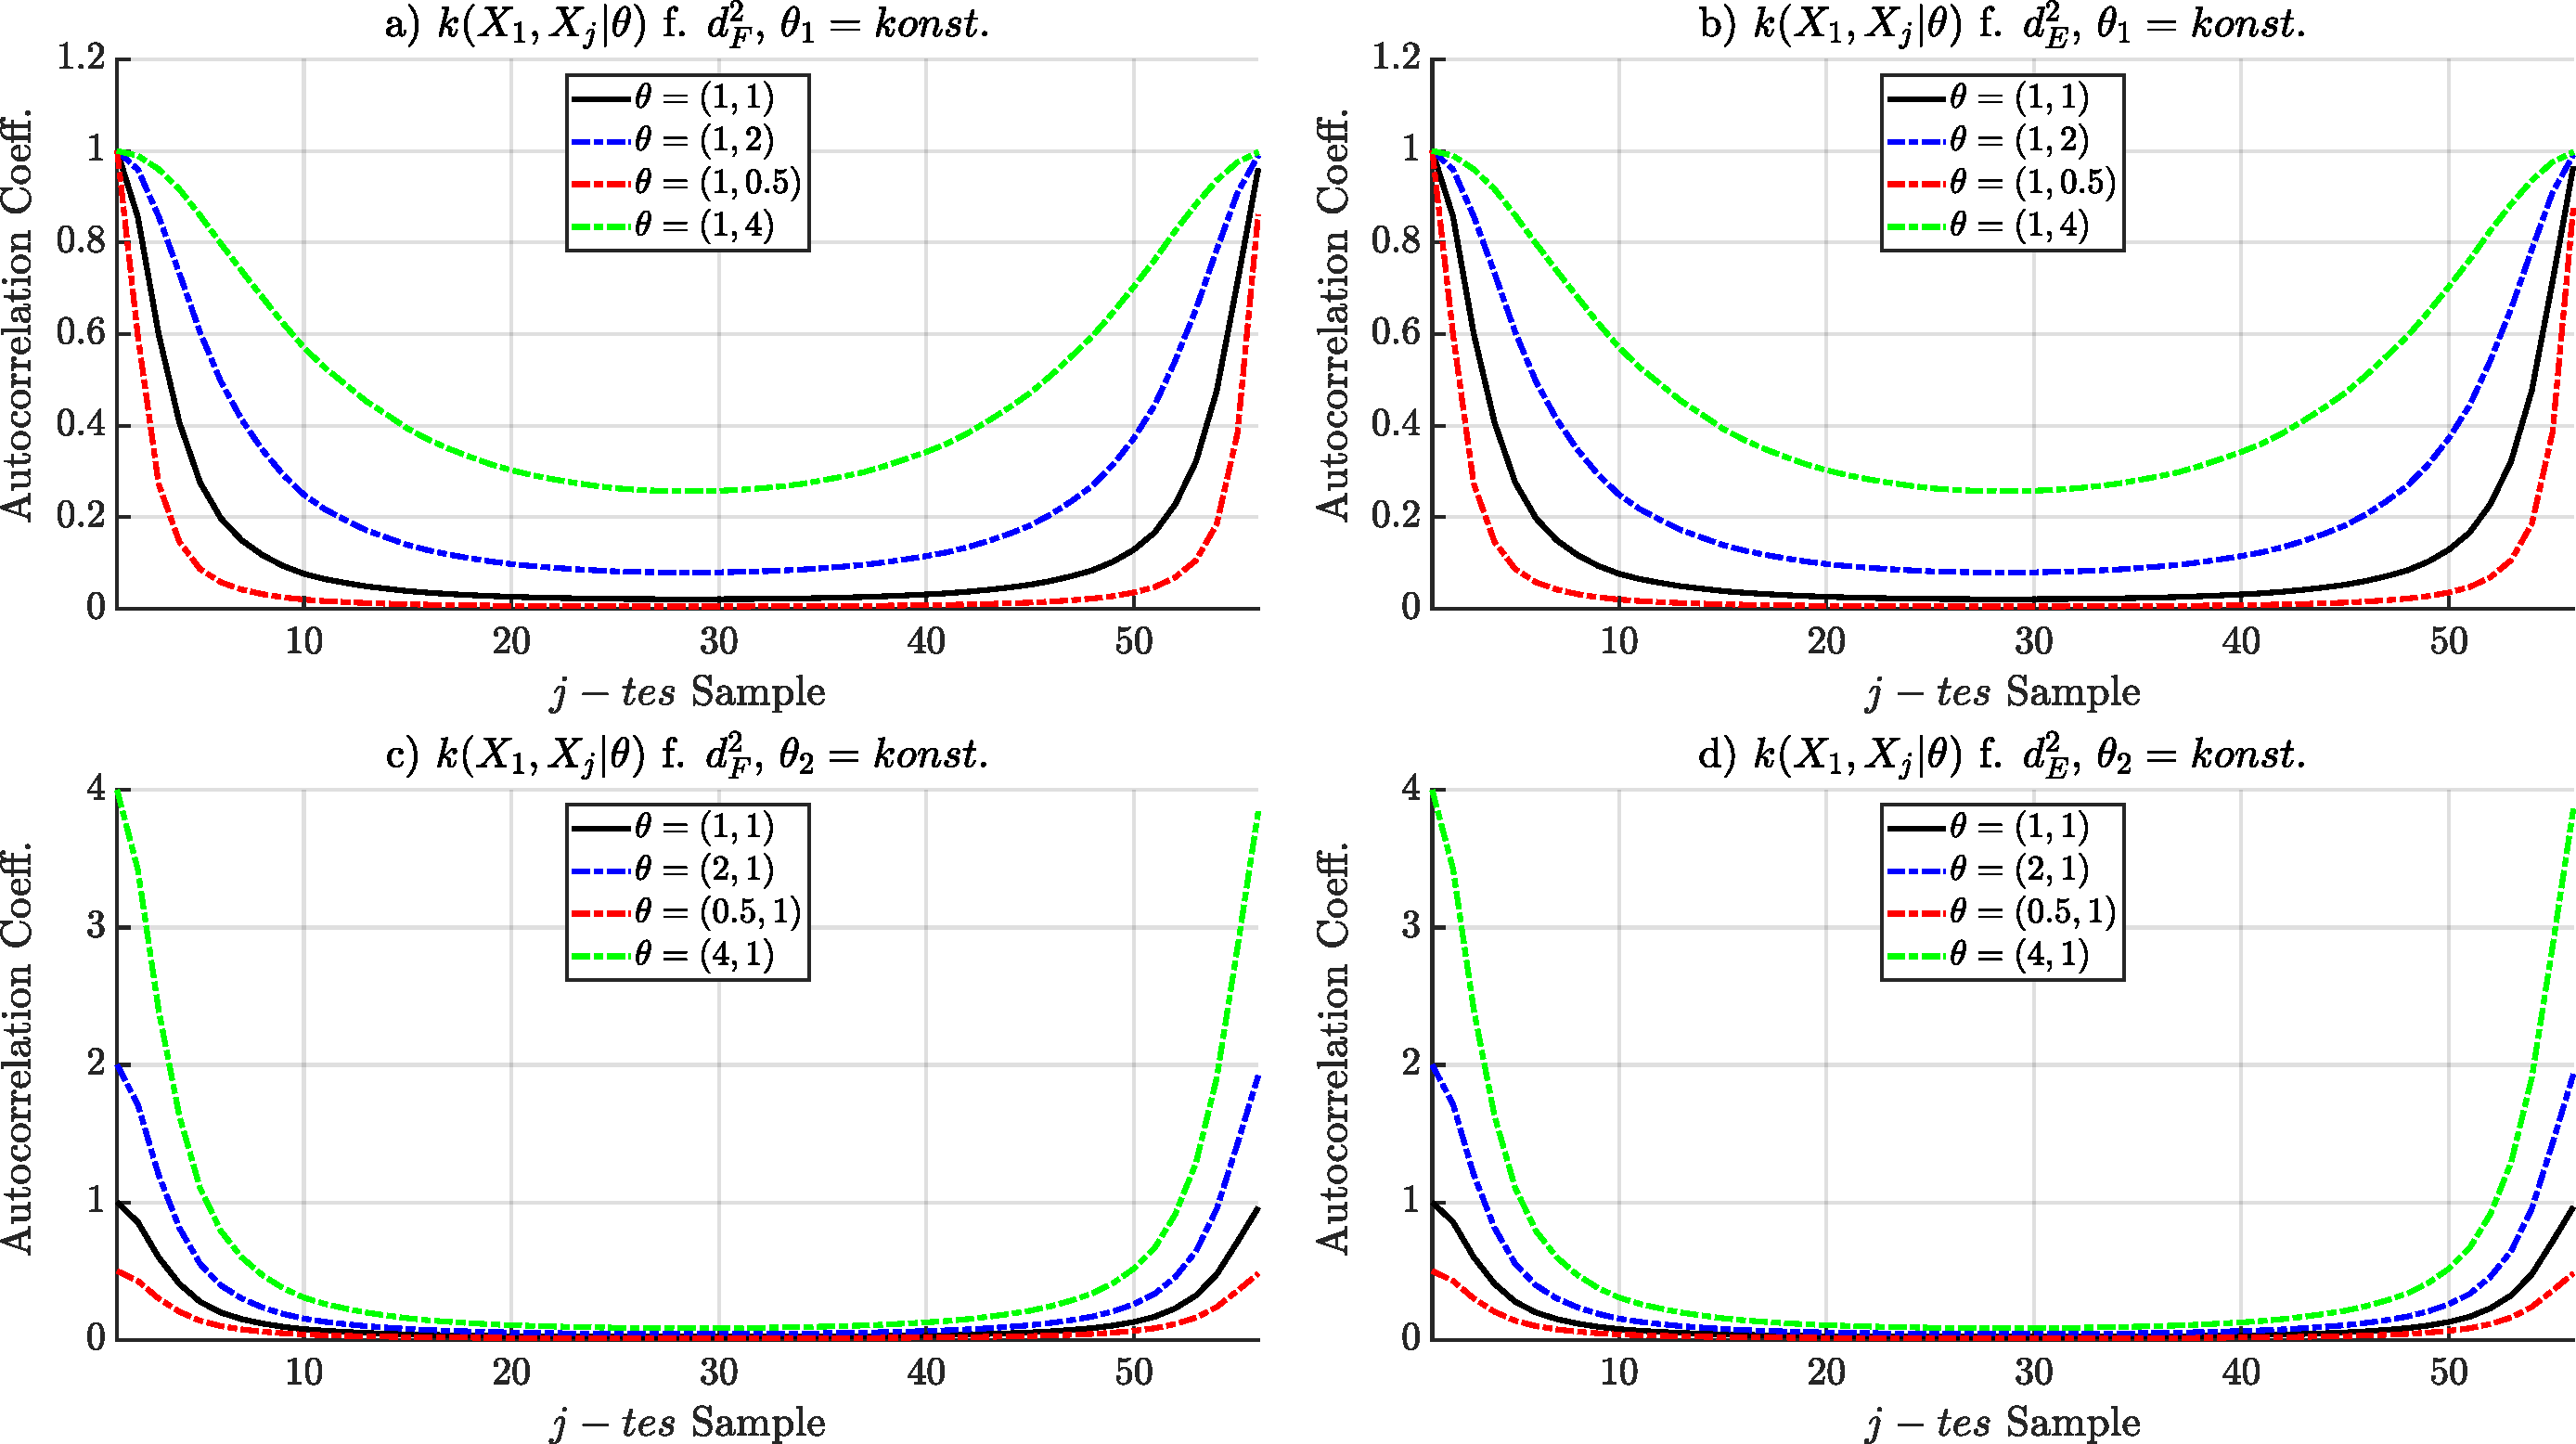
\includegraphics[width=\linewidth]{chapters/images/4-EuOExp/Vergleich-Kovarianzfunktionen}
\caption[Kovarianzfunktionen im Vergleich]{Kovarianzfunktionen im Vergleich für variierende Kernel-Parameter $\theta = (\sigma_f^2, \sigma_l)$ und $N_{Ref} = 56$ Referenzwinkel. Die Kovarianzfunktionen nach \autoref{eq:kfun} mit Frobenius-Norm nach \autoref{eq:df2} als Abstandsfunktion in den Abbildungen a) bzw. c) und mit euklidischer Norm nach \autoref{eq:de2innorm} in den Abbildungen b) bzw. d). Die Abbildungen a) und b) zeigen beide Funktionen mit variabler Längenskalierung $\theta_2 = \sigma_l$ und ausgeschalteter Höhenskalierung mit $\theta_1 = \sigma_f^2 = 1$. Vice versa sind beide Funktionen in den Abbildungen c) und d) gezeigt. Trainingsdaten basieren in a) und c) auf Matrizen. In b) und d) basieren Trainingsdaten auf Vektoren bzw. Skalare. Grafik nachempfunden aus \cite{Lang2014}.}
\label{fig:vergleich-kovarianzfunktionen}
\end{figure}


\clearpage
\begin{figure}[tph]
\centering
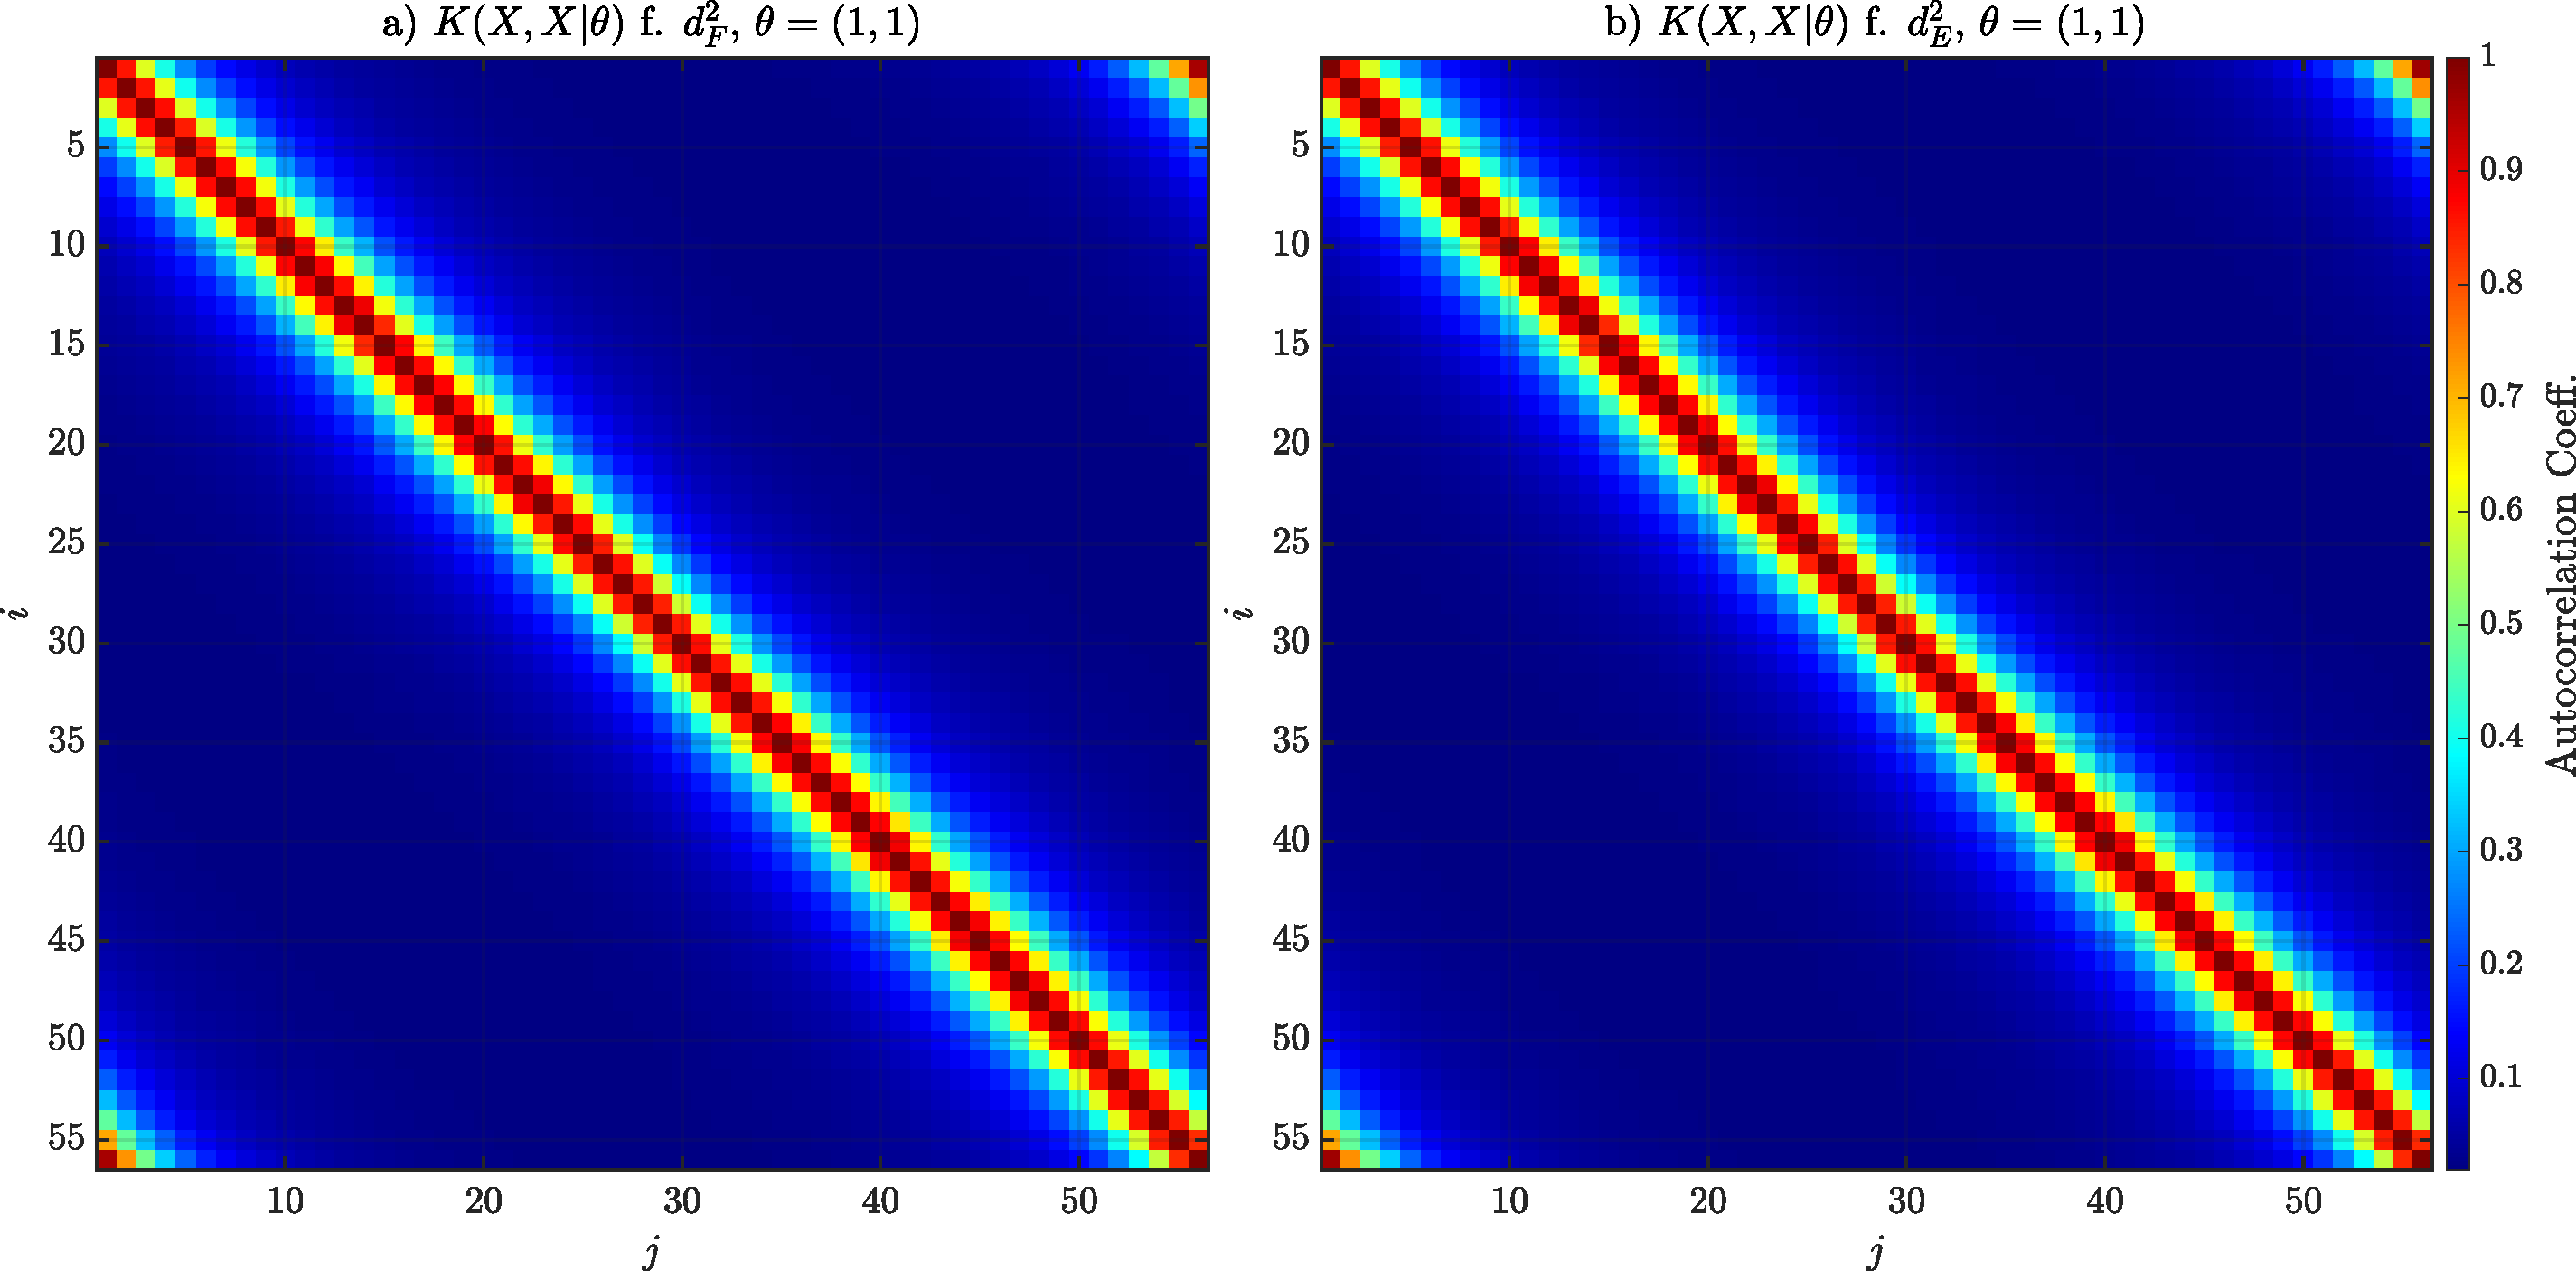
\includegraphics[width=\linewidth]{chapters/images/4-EuOExp/Vergleich-Kovarianzmatrizen}
\caption[Gegenüberstellung der Kovarianzmatrizen]{Gegenüberstellung der Kovarianzmatrizen bei ausgeschalteter Längen- und Höhenskalierung mit $\theta = (1,1)$ und $N_{Ref} = 56$ Referenzwinkel. In Abbildung a) nach Kovarianzfunktion mit Frobenius-Norm als Abstandsfunktion und in Abbildung b) mit euklidischen Abstand, siehe \autoref{eq:kfun}. In a) basieren Trainingsdaten auf Matrizen in b) auf Vektoren bzw. Skalare.}
\label{fig:vergleich-kovarianzmatrizen}
\end{figure}


\clearpage
\begin{figure}[tph]
\centering
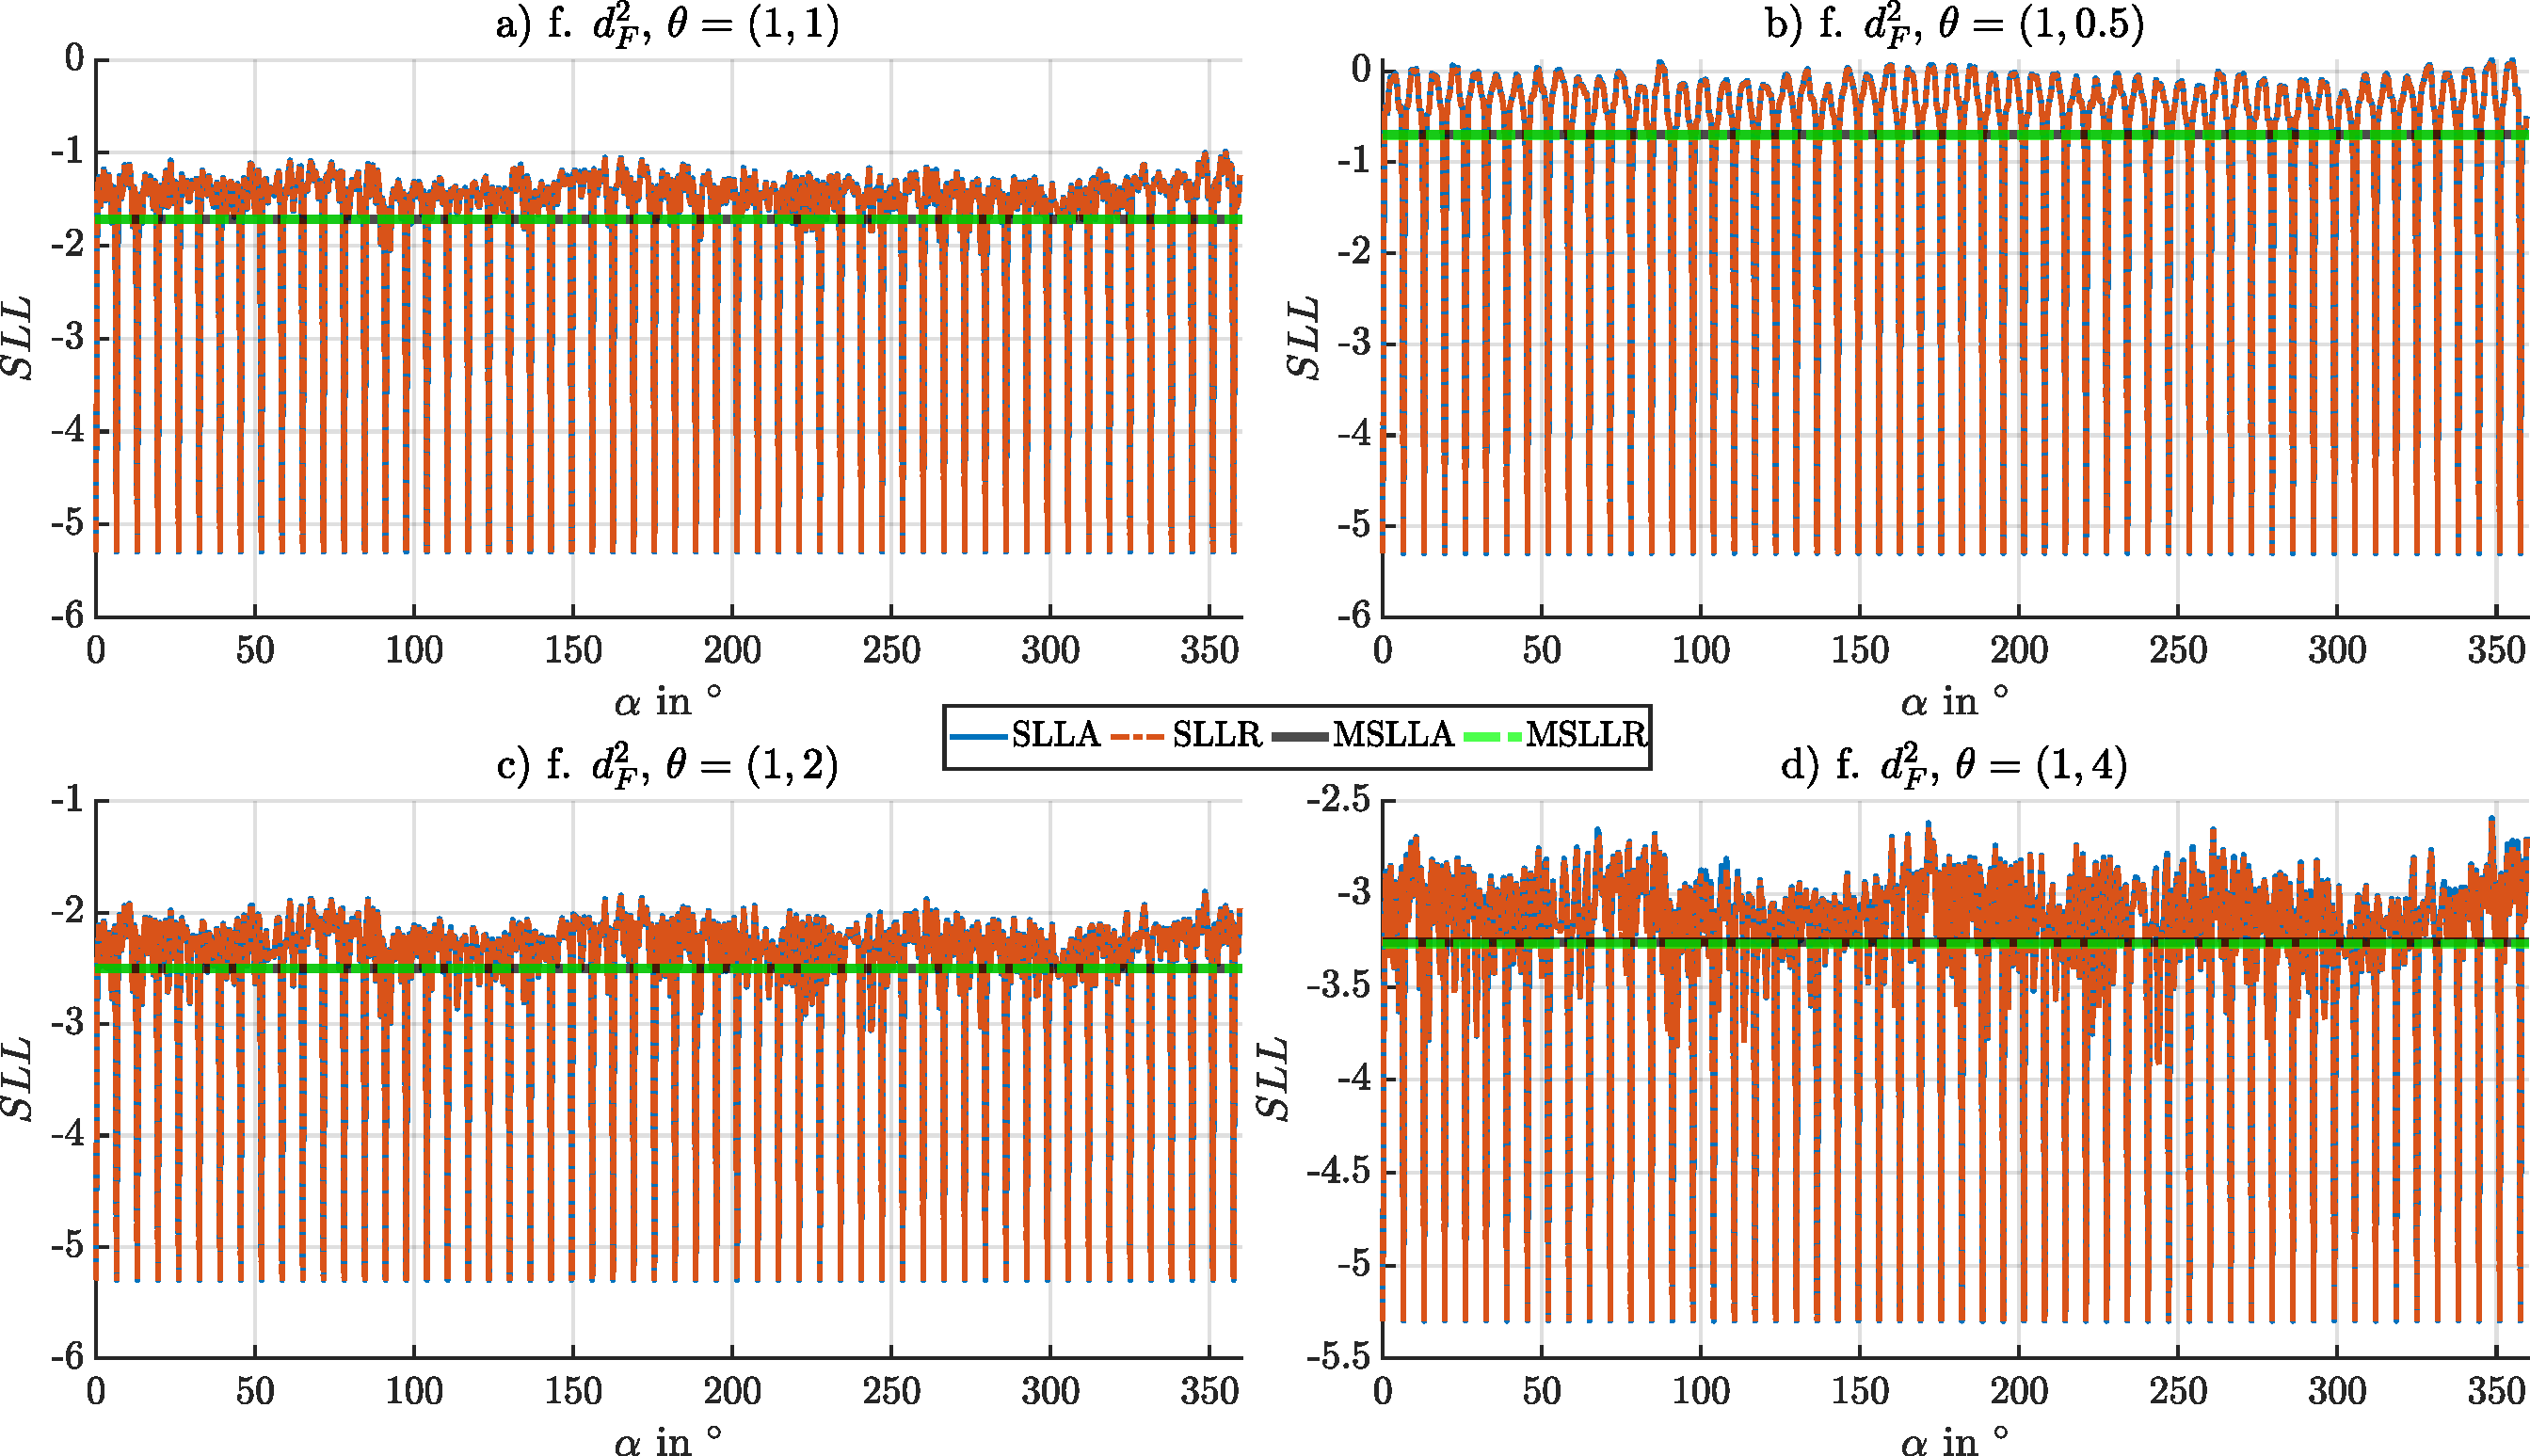
\includegraphics[width=\linewidth]{chapters/images/4-EuOExp/Vergleich-QFC-SLL}
\caption[Modellgeneralisierung mit Frobenius-Norm als Abstandfunktion]{Modellgeneralisierung mit Frobenius-Norm als Abstandfunktion nach \autoref{eq:kfun} und Trainingsdaten basierend auf Matrizen für $N_{Ref} = 56$ Referenzwinkel. Die Berechnungen zur Modellgeneralisierung erfolgten mit einem Testdatensatz für eine volle Rotation des Gebermagneten mit $720$ gleichverteilten Simulationswinkeln bei einer Winkelauflösung von $\SI{0,5}{\degree}$. Die Position des Sensors und die Magnetverkippung sind in beiden Datensätzen identisch. Variiert wurde die Längenskalierung $\theta_2 = \sigma_l$ bei ausgeschalteter Höhenskalierung $\theta_1 = \sigma_f^2 = 1$ der Kovarianzfunktion. Die Modellgeneralisierung wird über den standardisierten logarithmischen Verlust (engl. Loss) $SLL$ a. u. des Modells bewertet \cite{Rasmussen2006}. In Bezug auf Winkel (engl. Angle) mit $SLLA$ und Radius $SLLR$. Als Schwellwertkriterium dient die Mittlung (engl. Mean) der beiden Verluste zu $MSLLA$ und $MSLLR$ nach \autoref{eq:bayesopt}. Das Rauschniveau ist konstant mit $\sigma_n^2 = 10^{-6}$.}
\label{fig:vergleich-qfc-sll}
\end{figure}


\clearpage
\begin{figure}[tph]
\centering
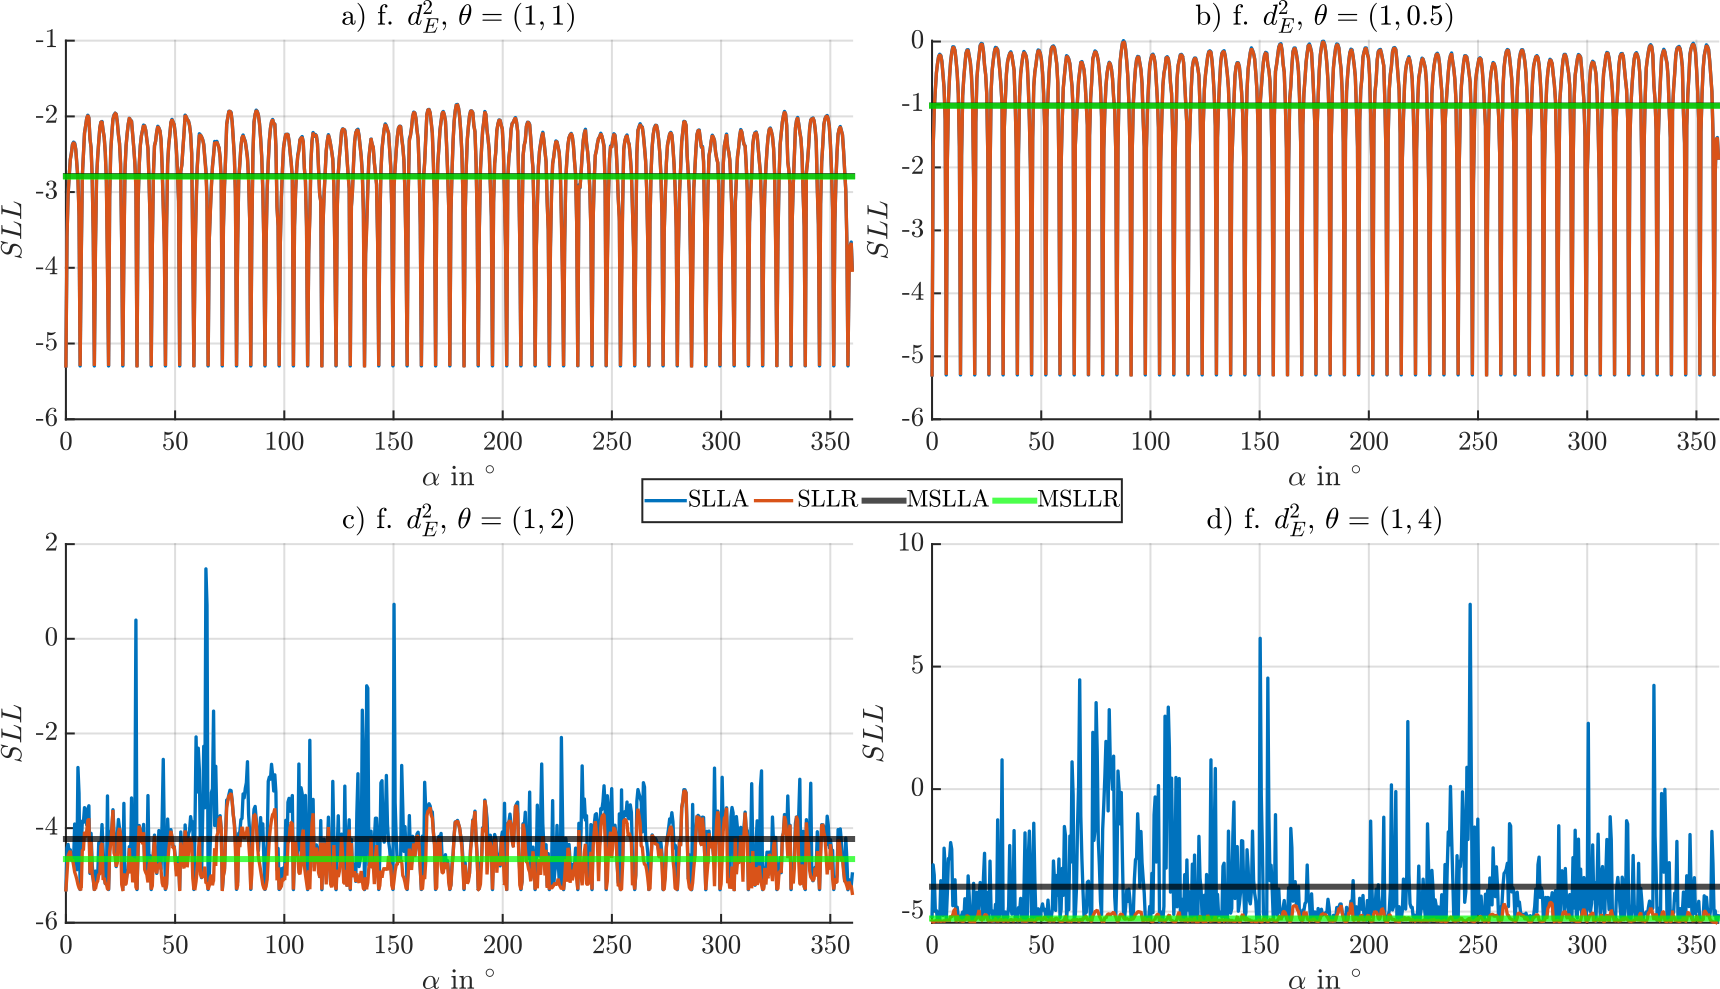
\includegraphics[width=\linewidth]{chapters/images/4-EuOExp/Vergleich-QFCAPX-SLL}
\caption[Modellgeneralisierung mit euklidischer Abstandsfunktion]{Modellgeneralisierung mit euklidischer Abstandsfunktion nach \autoref{eq:kfun} und Trainingsdaten basierend auf Vektoren bzw. Skalare für $N_{Ref} = 56$ Referenzwinkel. Die Berechnungen zur Modellgeneralisierung erfolgten mit einem Testdatensatz für eine volle Rotation des Gebermagneten mit $720$ gleichverteilten Simulationswinkeln bei einer Winkelauflösung von $\SI{0,5}{\degree}$. Die Position des Sensors und die Magnetverkippung sind in beiden Datensätzen identisch. Variiert wurde die Längenskalierung $\theta_2 = \sigma_l$ bei ausgeschalteter Höhenskalierung $\theta_1 = \sigma_f^2 = 1$ der Kovarianzfunktion. Die Modellgeneralisierung wird über den standardisierten logarithmischen Verlust (engl. Loss) $SLL$ a. u. des Modells bewertet \cite{Rasmussen2006}. In Bezug auf Winkel (engl. Angle) mit $SLLA$ und Radius $SLLR$. Als Schwellwertkriterium dient die Mittlung (engl. Mean) der beiden Verluste zu $MSLLA$ und $MSLLR$ nach \autoref{eq:bayesopt}. Das Rauschniveau ist konstant mit $\sigma_n^2 = 10^{-6}$.}
\label{fig:vergleich-qfcapx-sll}
\end{figure}
\clearpage

